%\documentclass[12pt,preprint]{aastex6}
\documentclass[12pt]{article}

\bibliographystyle{aasjournal}

\usepackage{aas_macros} % need this because not using aastex or emulateapj
\usepackage{graphicx}
\usepackage[suffix=]{epstopdf}
\usepackage{natbib}
\usepackage{amsmath}
%\usepackage{url}
\usepackage{xspace}
\usepackage{fullpage}

%    Make Scientific Notation
\providecommand{\e}[1]{\ensuremath{\times 10^{#1}}}

% make the word Kepler italicized
\newcommand{\Kepler}{\textsl{Kepler}\xspace}

\begin{document}
%%%%%%%%%%%%%%%%%%%%%%

%Measuring Stellar Rotation with K2

\title{\vspace{-0.5in}Scientific/Technical/Management}
\date{}

\maketitle


% shrink up the space between the "title" and first section heading
\vspace{-1in}

%%%%%%%%%%%%%%%%%%%
\section{Introduction}

%% uhoh, i was about to send up an entire introduction... maybe we should coordinate more about writing sections! :)


Among the key observational properties of main sequence stars in our galaxy, age is the most difficult to determine. Traditionally, fitting isochrones to cluster stars was one of the only precise methods for measuring ages, and was impossible for the majority of isolated field stars. Methods such as asteroseismology and measuring Li abundances require time intensive observations for each target and are not capable of producing the large quantity of ages needed for exoplanet and galactic population studies. To improve our understanding of star and planet formation and evolution, as well as the history of the Milky Way, we must be able to constrain the ages of low-mass stars like the Sun in the galactic field.

Fortunately nature has provided a power means to determine ages for main sequence stars via their rotation. Angular momentum is carried away though magnetically driven stellar winds, which slows the star's rotation over cosmic time. This rotation-based ``clock'' is known as {\it gyrochronology}. Cool spots on the star's surface rotate in-to and out-of view, creating small amplitude ($\sim$1\%) quasi-periodic changes in the stellar brightness. While rotation periods have previously been laboriously measured from starspot-induced flux modulations for hundreds of stars, space-based photometric surveys have opened the door to homogeneous ensemble measures of stellar rotation, and therefore age.
{\bf With the precise, long-duration light curves available from the \Kepler/K2 mission, we can determine the rotation periods and ages for nearly 100,000 main sequence field stars.}
%Stellar rotation periods are are the most promising tool for constraining the ages of field stars.

The \Kepler mission broke new ground by producing rotation periods for tens-of-thousands of field stars within a single $\sim$110 sq deg field of view, and discovered a surprising bimodal distribution of rotation periods. Two competing explanations have arisen for this mysterious feature: a bimodal age distribution for nearby stars, or a new subtlety in stellar angular-momentum-loss mechanisms. Detailed calibrations of gyrochronology models with the \Kepler rotation sample also revealed the need for samples of stars with a wider range of ages and compositions. Fortunately the ongoing \Kepler extended mission, K2, has currently produced light curves from 14 additional fields throughout the Galaxy.

To enable studies of stellar ages from rotation periods with K2, we propose to:

{\bf 1.} Measure accurate rotation periods for every available K2 target, using new statistical methods we have developed to cope with significant instrumental systematics in the K2 data. This value-added dataset will improve the \Kepler data legacy for field stars, and provide a critical training set for the TESS mission. 

{\bf 2.} Produce updated gyrochronology relations based on a wider range of field star ages, and additional open clusters within the K2 fields.

{\bf 3.} Determine the origin of the mysterious rotation period bimodality discoverd with \Kepler by tracing the rotation period distribution in each K2 field, and out to further distances utilizing public Gaia data.

{\bf 4.} Measure the star formation history within each K2 field using a new Bayesian age-dating system.



\clearpage



%%%%%%%%%%%%%%%%%%%
\section{Scientific Motivation}
Galactic archaeology and exoplanet populations are two rapidly accelerating
fields of interest within astronomy.
Although seemingly unconnected, these two fields are linked by a mutual
requirement for precise stellar parameters.
To galactic archaeologists, ages and elemental abundances are the most
important parameters.
Indeed, most galactic archaeology surveys target exactly these properties.
For exoplaneteers, masses and radii have historically been the most important
stellar parameters for understanding planetary systems. With a
growing number of planet hosts with precise masses and radii, attention is turning
toward other parameters such as ages to under the history and evolution of these systems. 
Age is therefore a fundamental stellar parameter of great interest to two large
communities of astronomers. However it is a difficult attribute to measure for
main sequence F, G, K, and M stars in the field, in part because low-mass dwarfs do not move far on the Color-Magnitude
diagram (CMD) during their hydrogen burning lifetimes. Further,
competing stellar evolution models predict different ages for the same star.
%Asteroseismology, while a very precise age-dating tool, is not capable of
%producing the large quantity of ages needed for exoplanet and galactic
%population studies.
Of all the measurable properties for a large numbers of stars, rotation periods contain
the most information about stellar age, and provide the best leverage for advancing our knowledge of galactic archeology as well as exoplanet population demographics. 





%%%%%%%%%
\subsection{Rotation Periods from \Kepler and K2}
Previous ground-based efforts to constrain stellar rotation periods for single, isolated field stars have resulted in few measurements. Detecting rotation from Doppler line broadening requires obtaining medium- to high-resolution spectroscopy of individual targets, and can be subject systematic effects such as from limb darkening approximations \citep{collins1995}. These observations also require time on larger aperture telescopes to reach fainter magnitudes needed to study rotation from low-mass field stars, or for studying the entire mass range within stellar clusters. Ground-based photometric wide-field surveys overcome many of the difficulties in gather large samples of field stars or entire stellar clusters. However, long duration monitoring with relatively high cadence and high photometric precision is required to detect the small amplitude and slowly varying flux modulations from starspots. These campaigns typically yielded rotation samples of hundreds to $\sim$1000 stars \citep[e.g.][]{hartman2010,hartman2011}


Space-based photometry surveys designed for exoplanet transit searches such as \Kepler \citep{borucki2010} have produced a revolution in stellar rotation studies. The original \Kepler mission produced light curves up to four years in duration with $\sim$100 ppm precision at 30-minute cadence for more than 200,000 stars. From this remarkable dataset, more than 30,000 unique stellar rotation periods have been measured using a variety of time series analysis techniques such as the Lomb-Scargle Periodogram \citep{reinhold2013} and the Autocorrelation Function \citep[][]{mcquillan2014}.
This bounty of rotation periods has also allowed the first ensemble investigations in to stellar surface differential rotation \citep[e.g.][]{reinhold2013}, revealed stars with near solid-body rotation \citep{davenport2015a}, and highlighted the many degeneracies in disentangling starspot evolution and differential rotation \citep{aigrain2015}.


After hardware failures made observations of the original field impossible, an extended \Kepler mission was designed to observe many fields with $\sim$3 month durations. The K2 mission has observed fields spaced along the ecliptic plane, ranging from low galactic latitudes that include multiple open clusters, to high galactic latitudes that include many older field stars \citep{howell2014}. The K2 fields also include several benchmark stellar clusters including the Solar-age M67, the Pleiades and Hyades, and M35. To date K2 has released data from 10 distinct campaigns (or fields), including more than 252,000 targets, exceeding the original \Kepler mission. An additional 6 campaigns are currently scheduled. Importantly, K2 data quality has been demonstrated to approach that of the original \Kepler mission \citep{luger2016}, and has been successfully used to measure rotation periods for select targets such as open cluster stars \citep[e.g.][]{douglas2017}. 





%%%%%%%%%
\subsection{Age-Dating Field Stars with Rotation}

\citet{skumanich1972}
\citet{barnes2003,barnes2007}
the promise of gyrochronology is key, has ability to get ages with accuracy that rivals any other method (10\%). with Kepler/K2 is a mass production job, but with K2 new challenges in the data are lurking

\begin{figure}[!th]
\centering
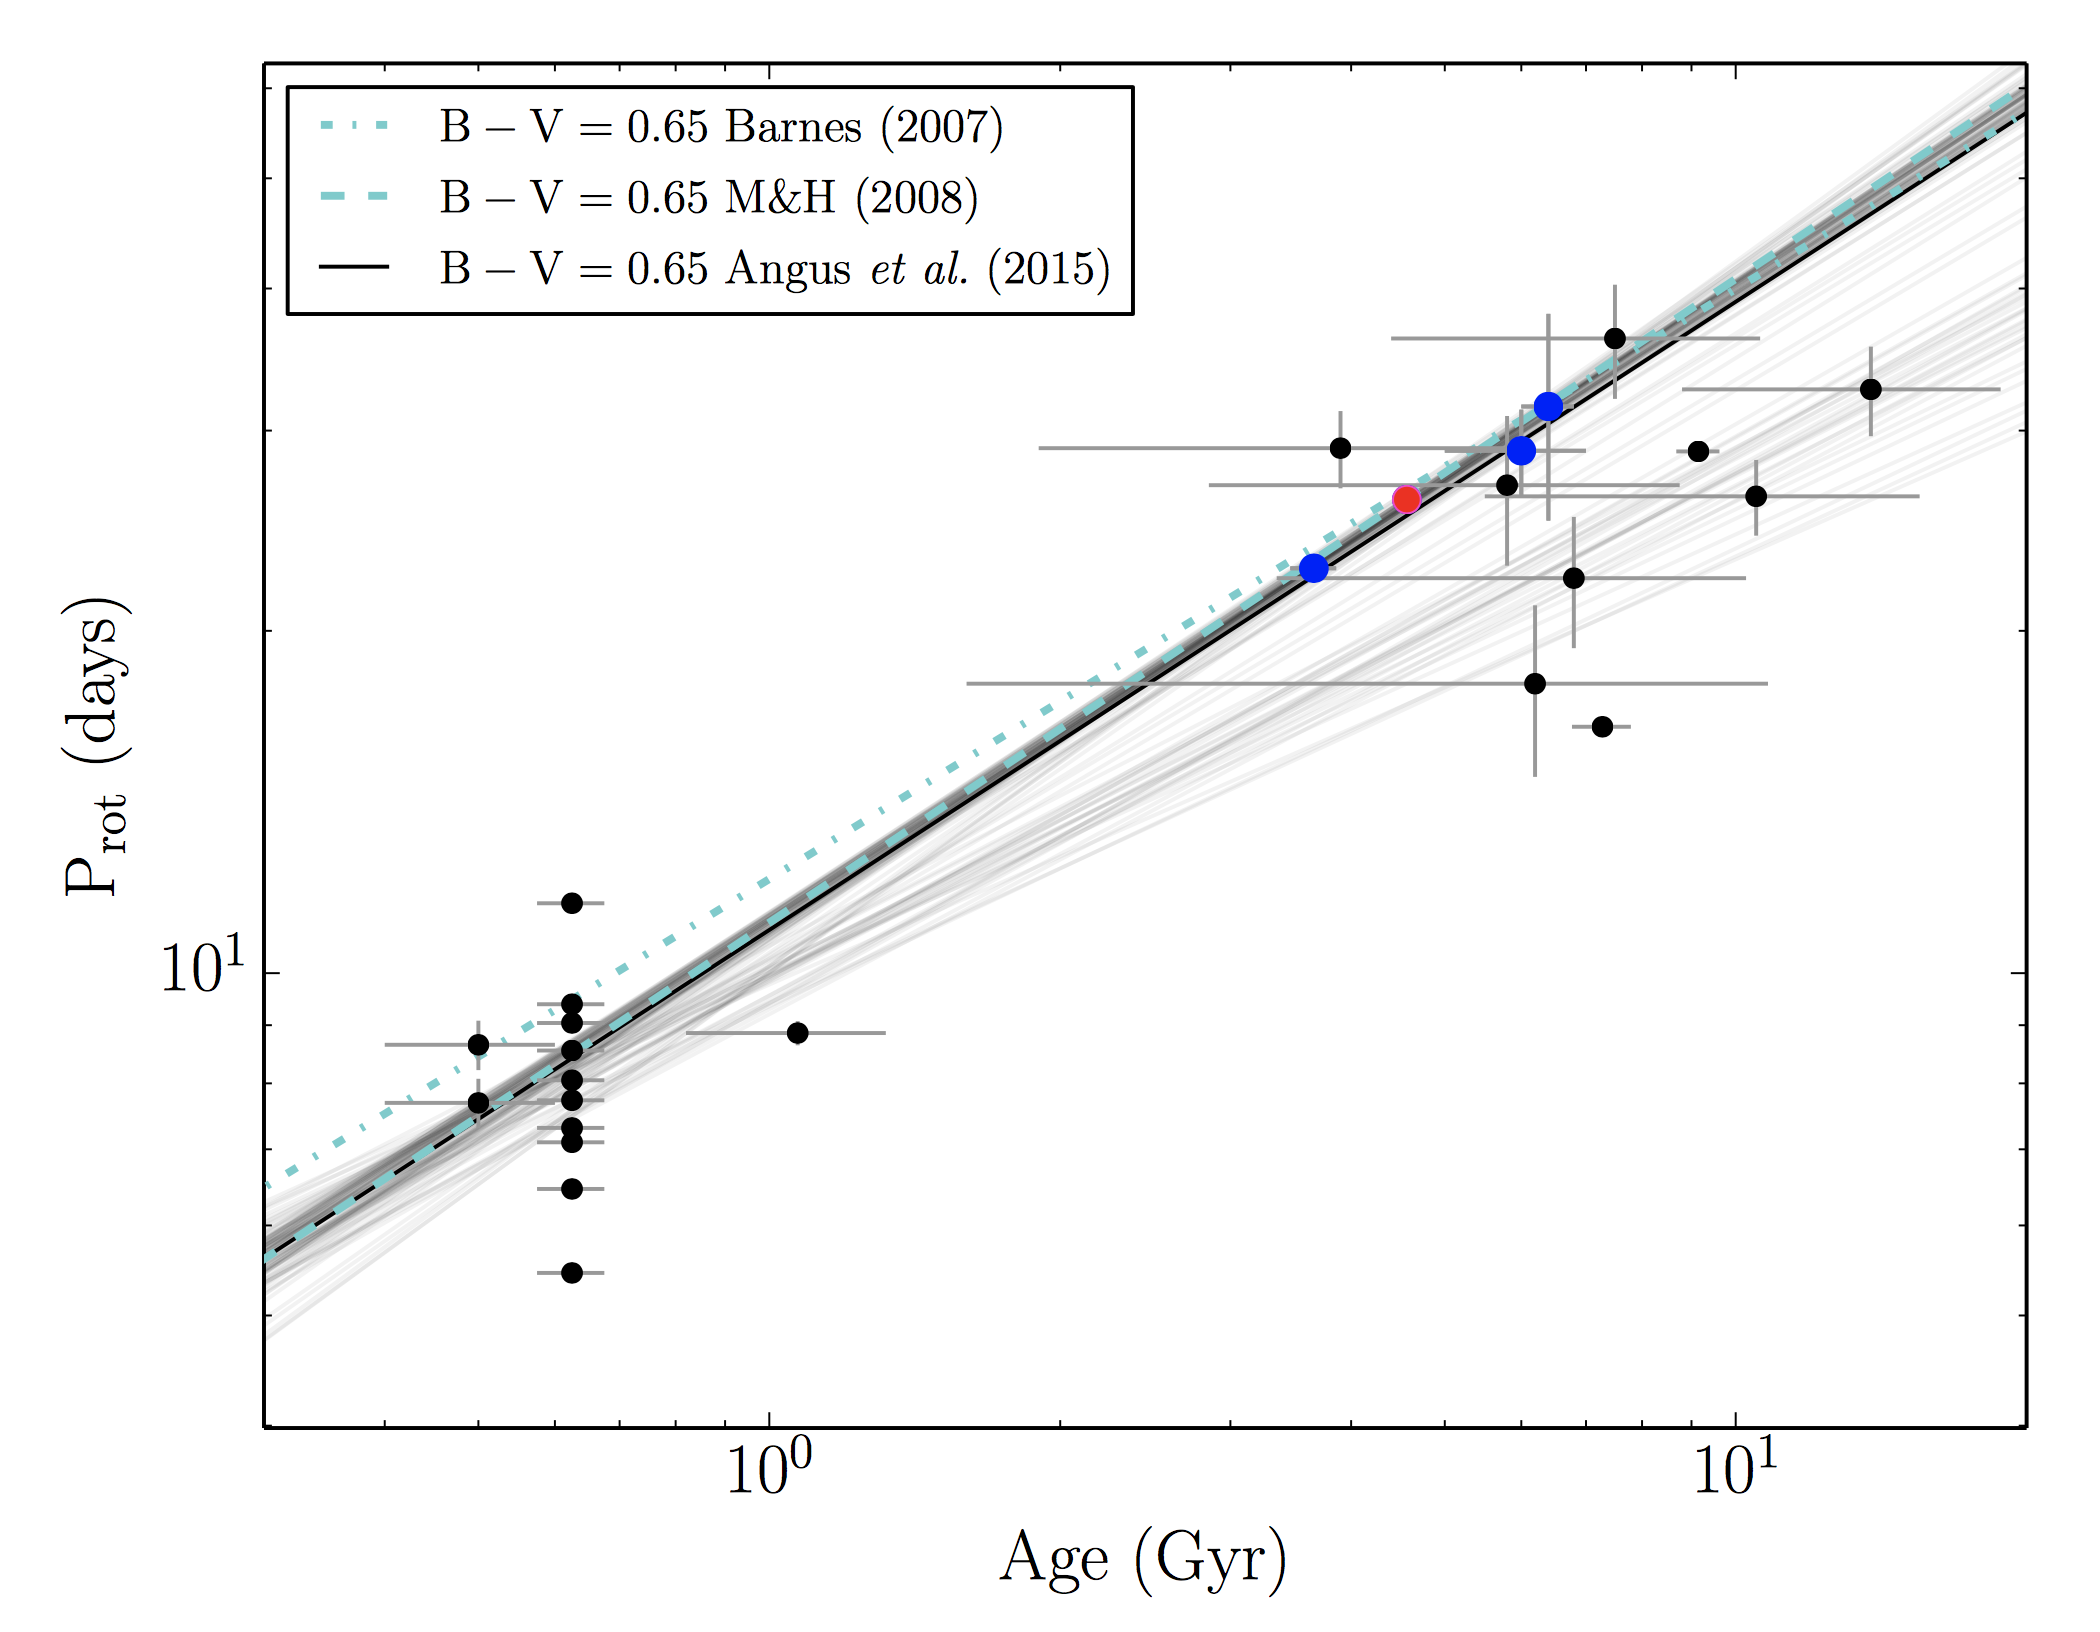
\includegraphics[width=4in]{angus2015_fig6.png}
\caption{figure 6 from \citet{angus2015}, showing new gyrochronology relation calibrated using \Kepler asteroseismic targets
}
\label{fig:gyro}
\end{figure}



%%%%%%%%%
\subsection{A Mysterious Period Bimodality}

Then this weird thing appeared, which is an open mystery - a bimodal period distribution - whoa \citep{mcquillan2013}. this was then extended to higher masses by \citet{davenport2017}. Explanations are either a break from single spin-down law (possibly from different initial periods, or some new physics maybe due to chemical abundances) or represents an age bimodality of local stars.

 Since this effect is seen only within 300pc so far (and only within Kepler data) due to sample properties, cannot be sure what spatial or compositional dependence this has, need a sample that spans a wider spatial area and more ages of stars

\begin{figure}[!th]
\centering
\makebox[\textwidth][c]{ % sloppy hack to make figure slightly overflow
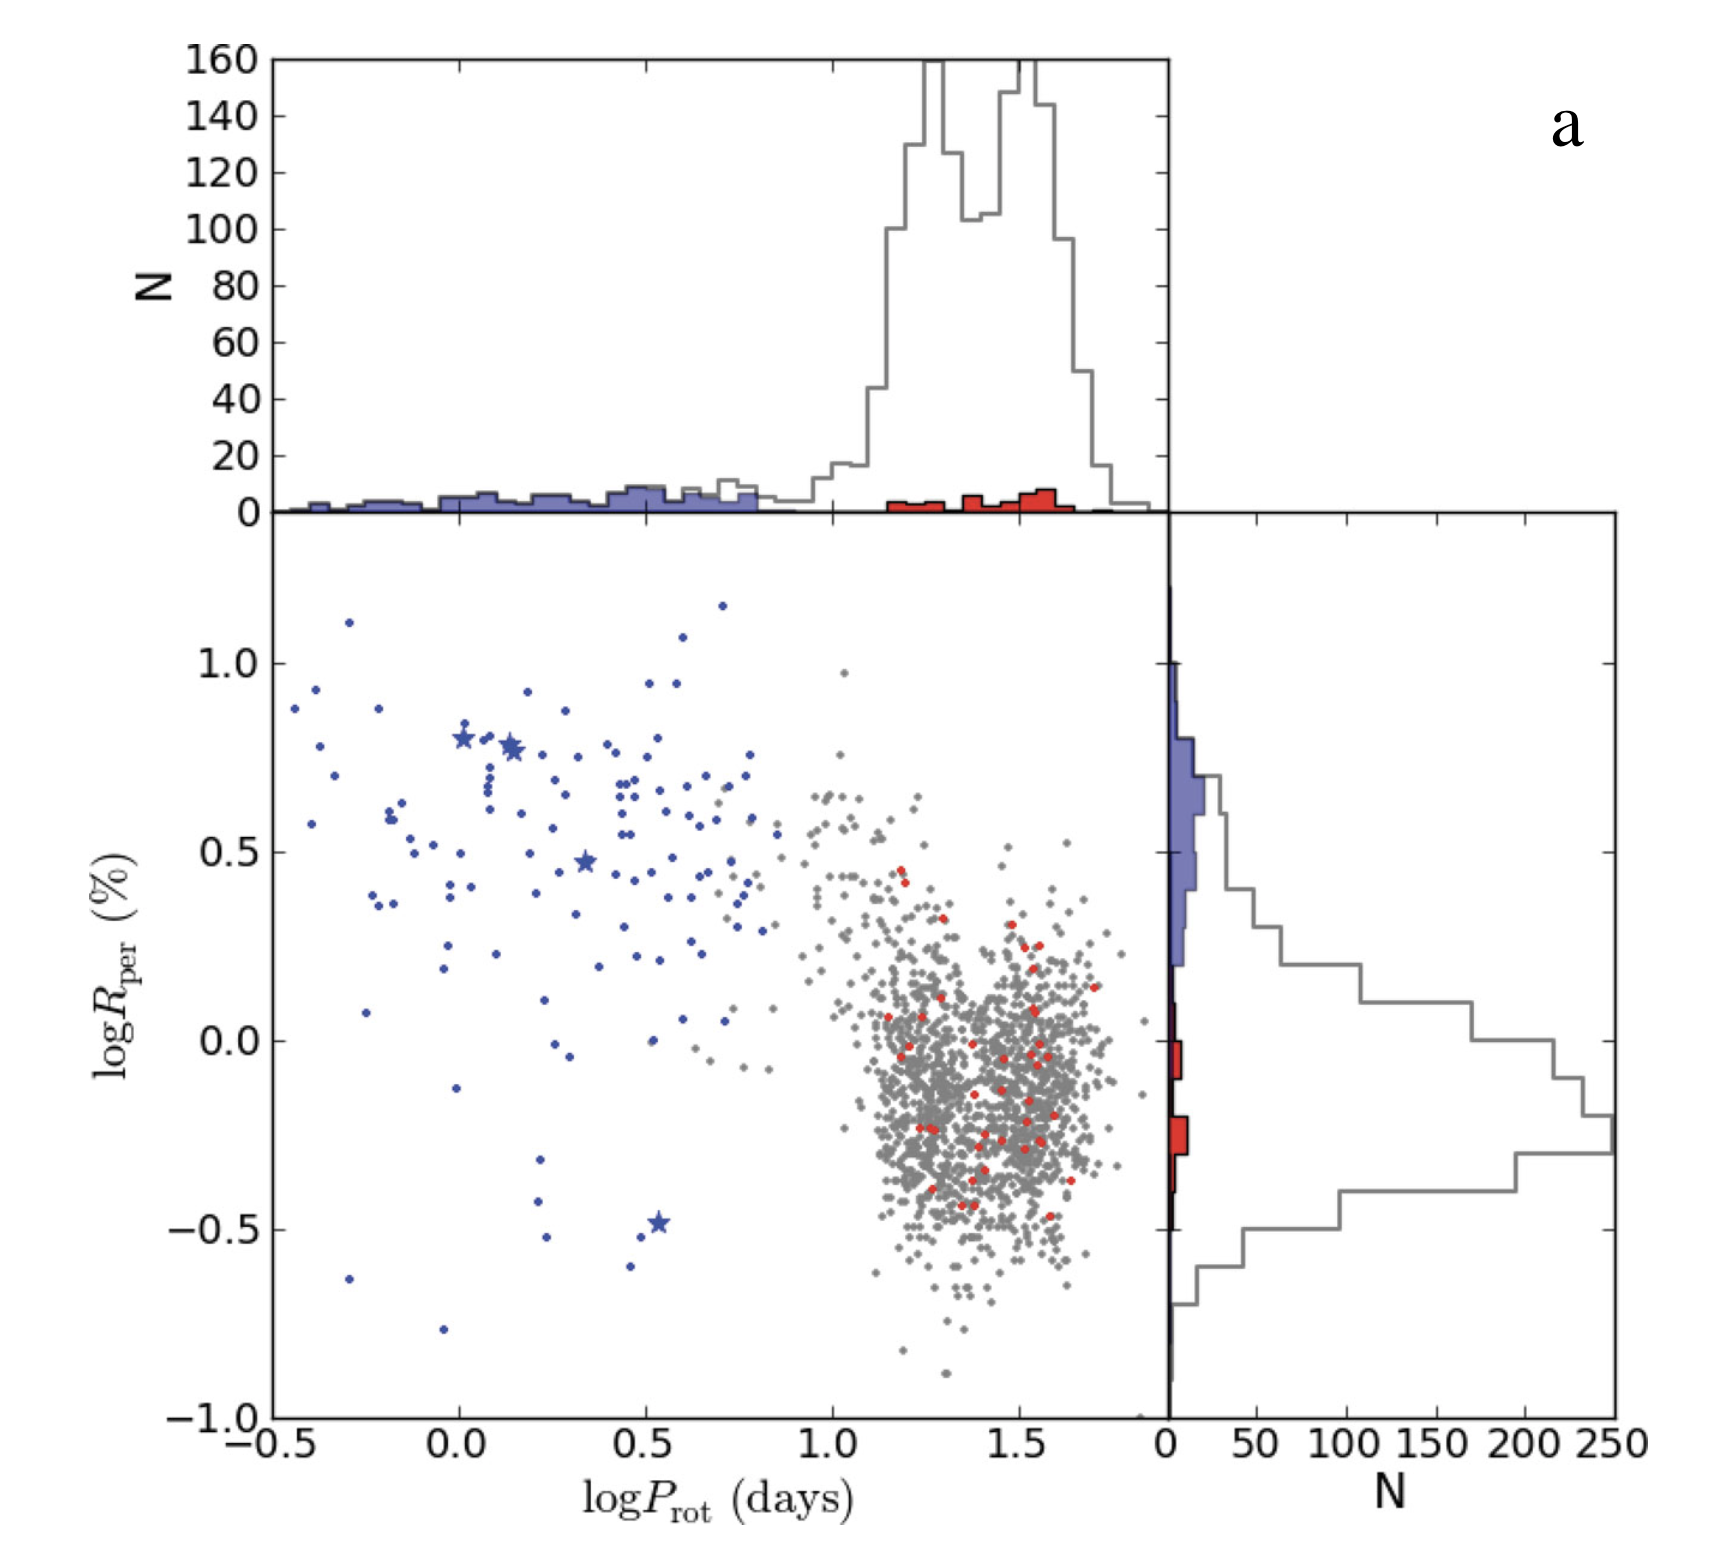
\includegraphics[width=3in]{mcquillan2013_fig9.png}
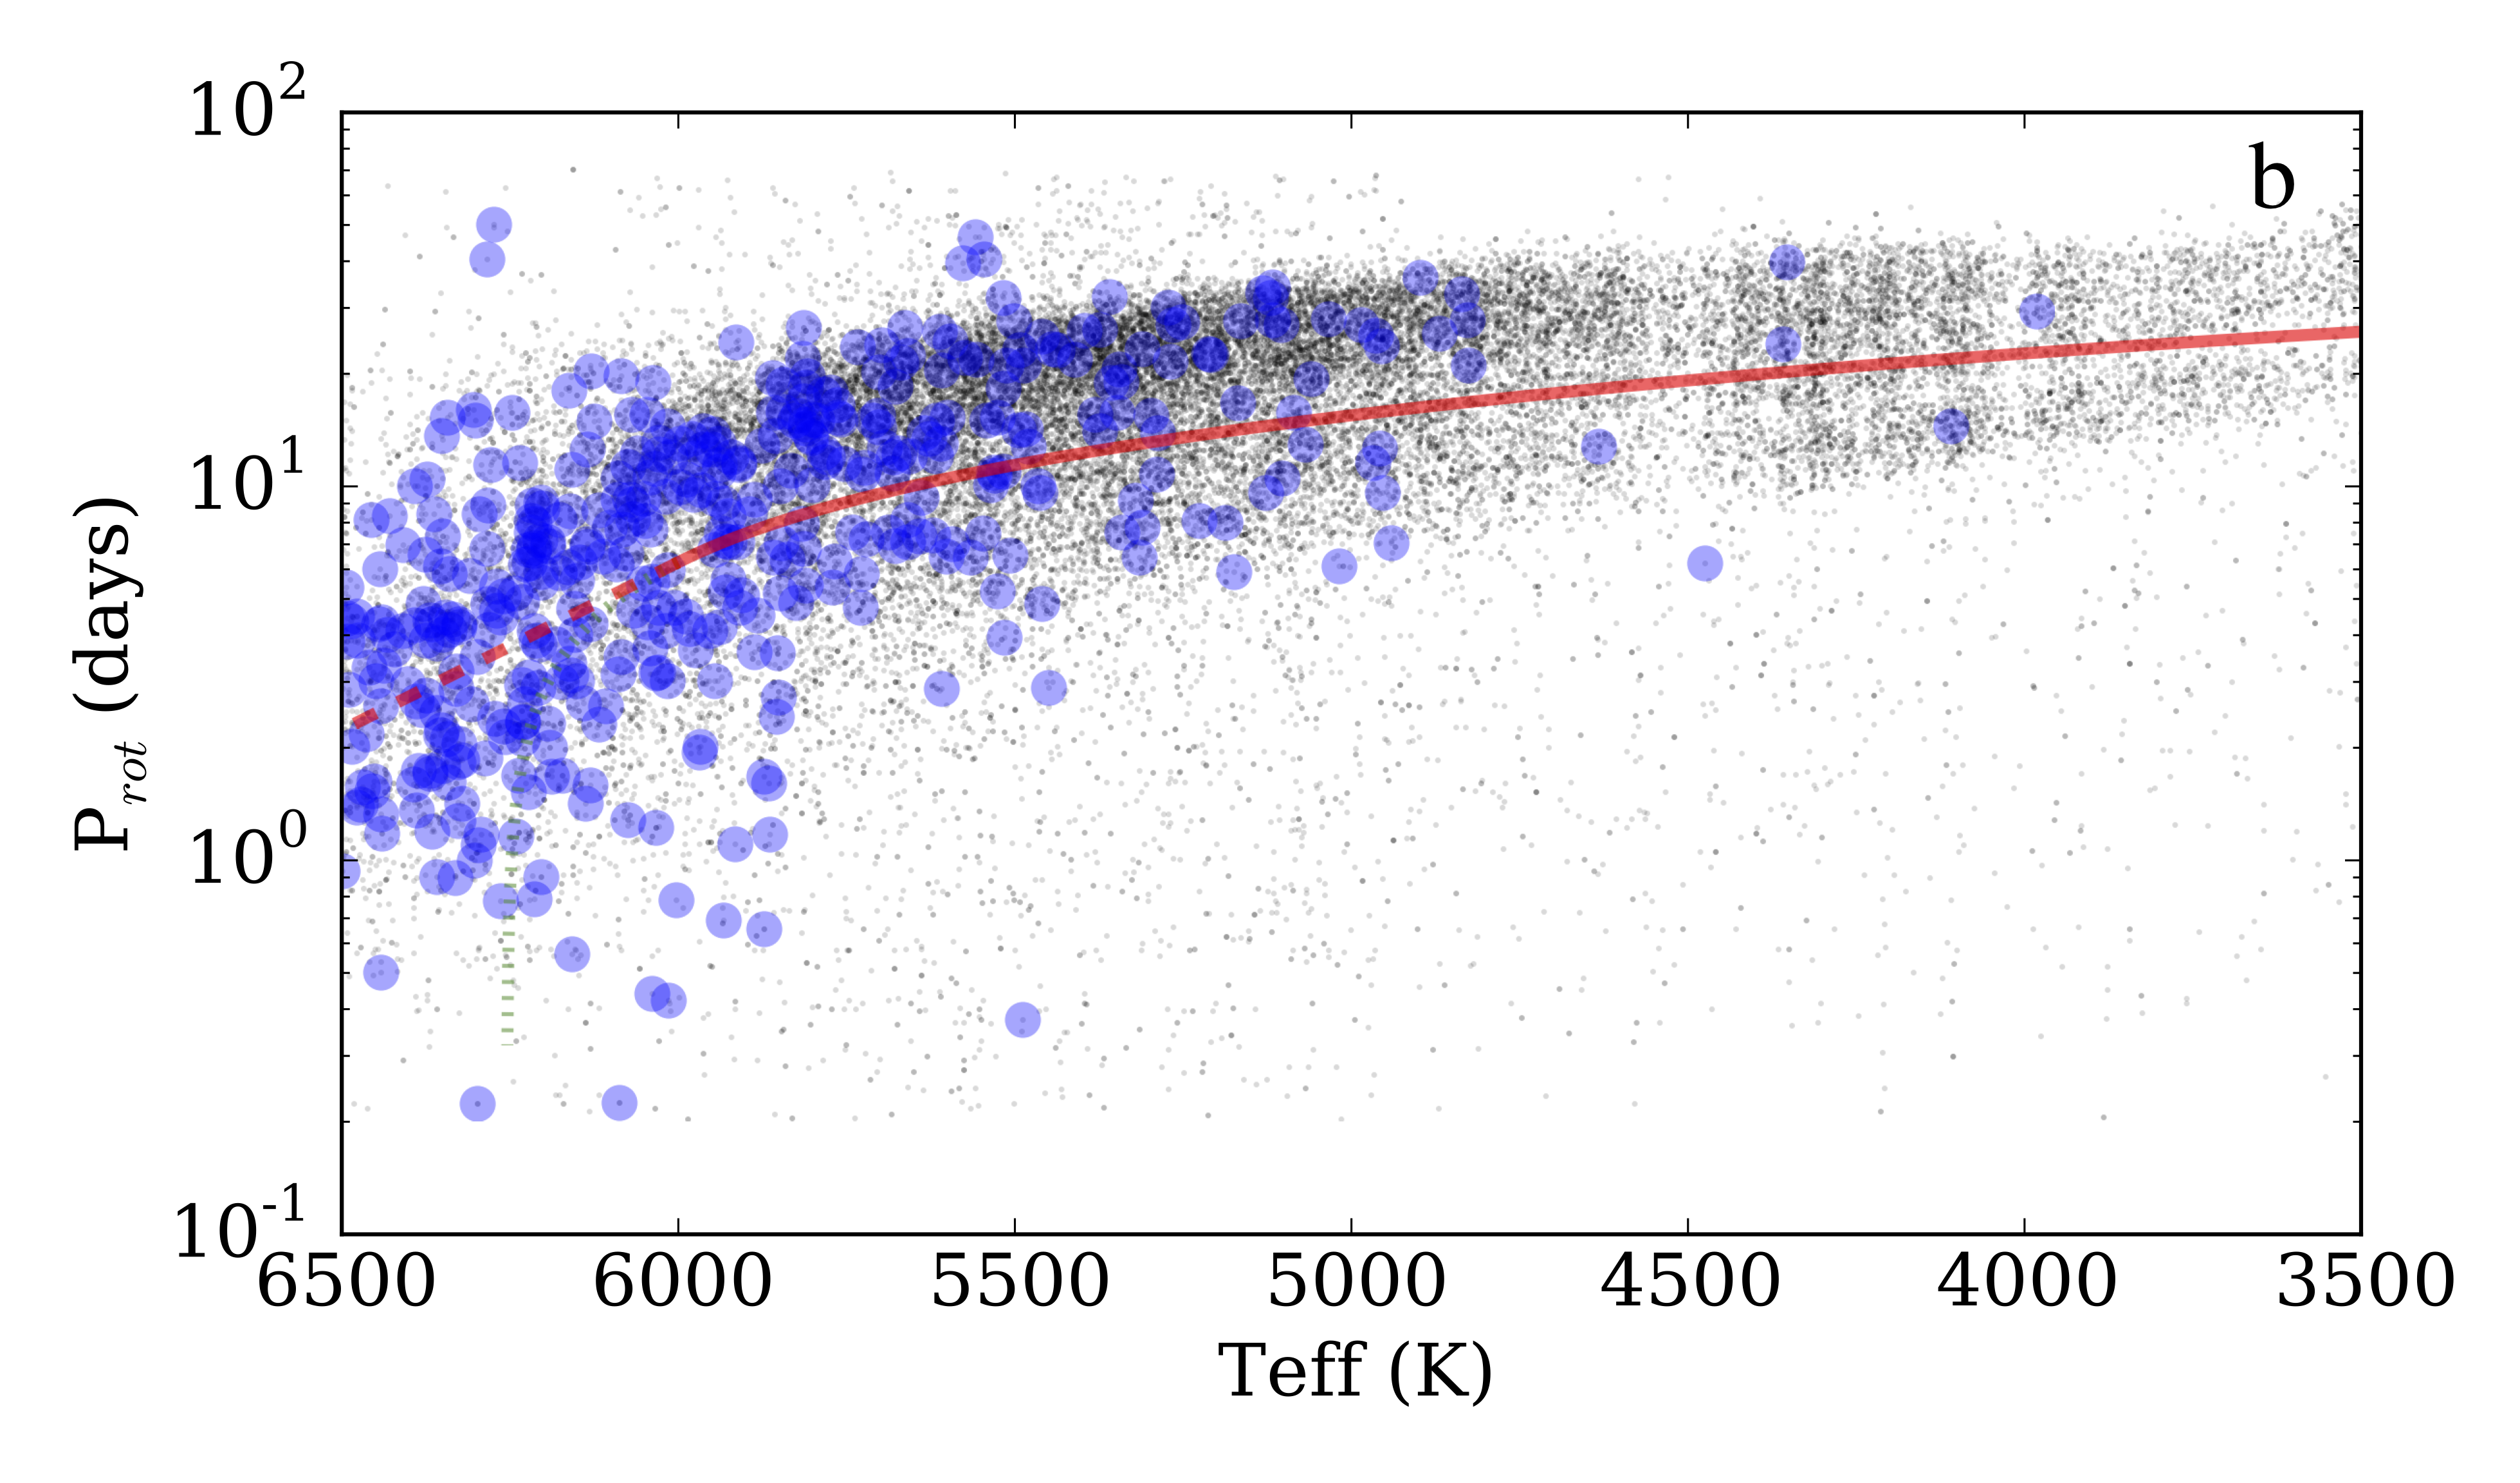
\includegraphics[width=4in]{davenport2016_fig3}
}
\caption{
Left -- Figure 9 from \citet{mcquillan2013}; the discovery of a bimodality in rotation periods from \Kepler M dwarfs (middle panel).
Right -- Figure 3 from \citet{davenport2017}, showing all \Kepler rotation periods from \citet{mcquillan2014} (black dots), and main sequence stars with Gaia DR1 distances. The bimodality discovered for M dwarfs extends to G and K stars, and straddles  a 600 Myr ``gyrochrone'' (red line).
}
\label{fig:bimodal}
\end{figure}



%%%%%%%%%%%%%%%%%%%
\section{Proposed Research}
%%%%%%%%%
\subsection{Measuring Rotation from K2 Using the Systematics-Insensitive Periodogram }
we propose the first systematic study of stellar rotation periods from the K2 data.

this will include $\sim$XXXXX stars from Campaigns 0-16. This includes data for multiple stellar clusters that were taken as part of the Guest Observer program.

data will be reduced using SOME FLAVOR of K2 pipeline.


the \citet{angus2016} rotation period pipeline will then be applied to every light curve. we will generate and save every periodogram for potential follow-up analysis of differential rotation and multi-period systems

spurious signals from transits and flares will be filtered out (some smoothing or high-freq removed in the SIP?)

for stars with good period recovery, fourier fits will identify eclipsing binaries and pulsating systems (or something like this)


\begin{figure}[!th]
\centering
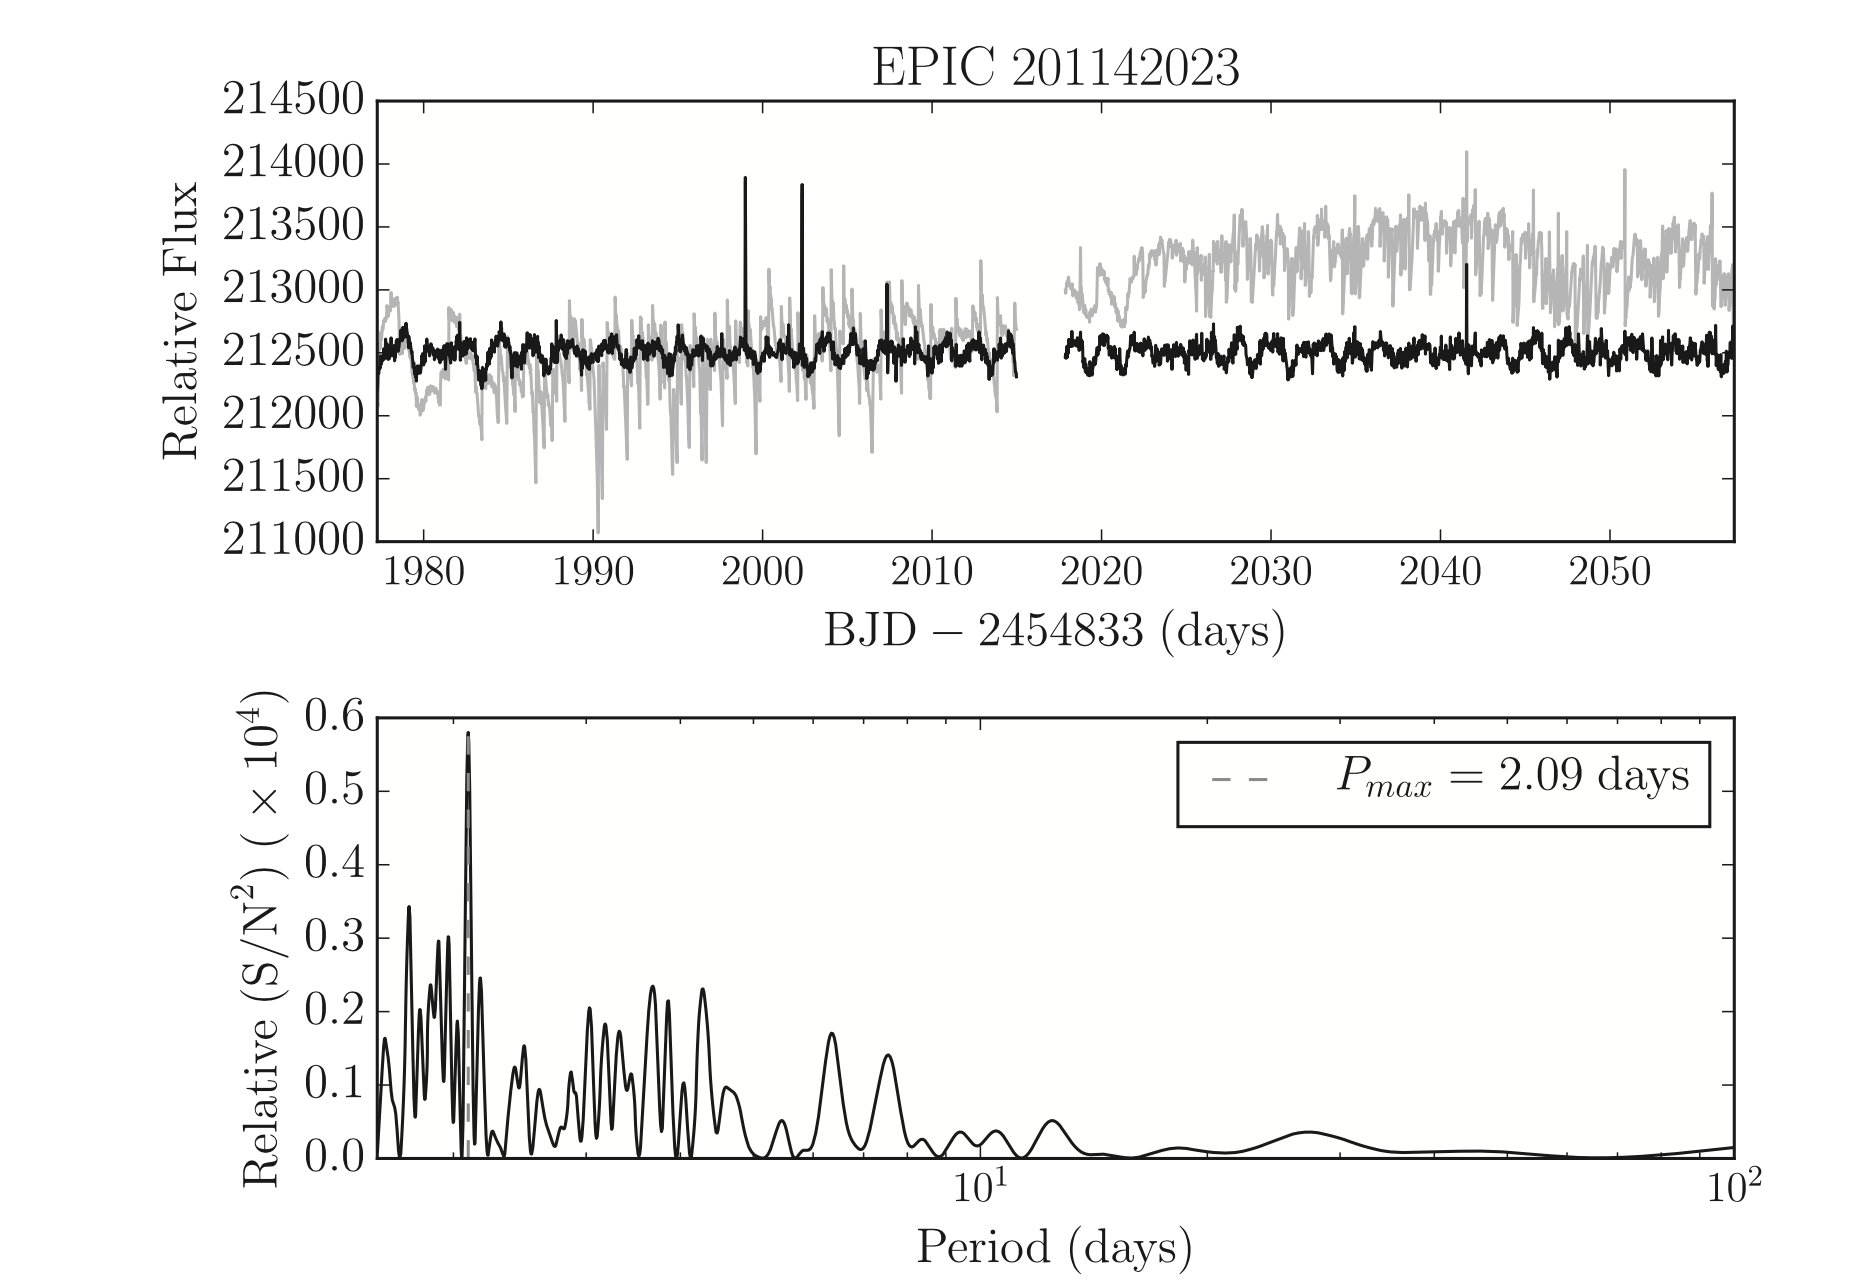
\includegraphics[width=4in]{angus2016_fig6.png}
\caption{
figure 6 from \citet{angus2016}, showing the processing of the light curve and resulting SIPeriodogram. more simple methods give erroneous periods for this object of either 3 days via ACF, or 59 days via normal Lomb-Scargle methods.
}
\label{fig:sip}
\end{figure}

The \Kepler rotation period catalog from \citet{mcquillan2014} found a yield of $\sim25\%$ of stars had measurable rotation periods using the Autocorrelation Function. From our sample of 252,000 available K2 targets, we expect to recover $\sim$63,000 new rotation periods, bringing the total \Kepler/K2 sample to $\sim$100,000.


%%%%%%%%%
\subsection{Exploring the Period Bimodality}
by combining our sample with the distances provided in the forthcoming Gaia DR2 catalog, we will be able to extend the methodology of \citet{davenport2017} to filter our subgiants and binary stars for our entire sample.

we then can make 3d exploration of period distribution, to see if the bimodality exists for all field stars near the sun.

the big goal here is to decide which explanation is correct!

\begin{figure}[!th]
\centering
\makebox[\textwidth][c]{ % sloppy hack to make figure slightly overflow
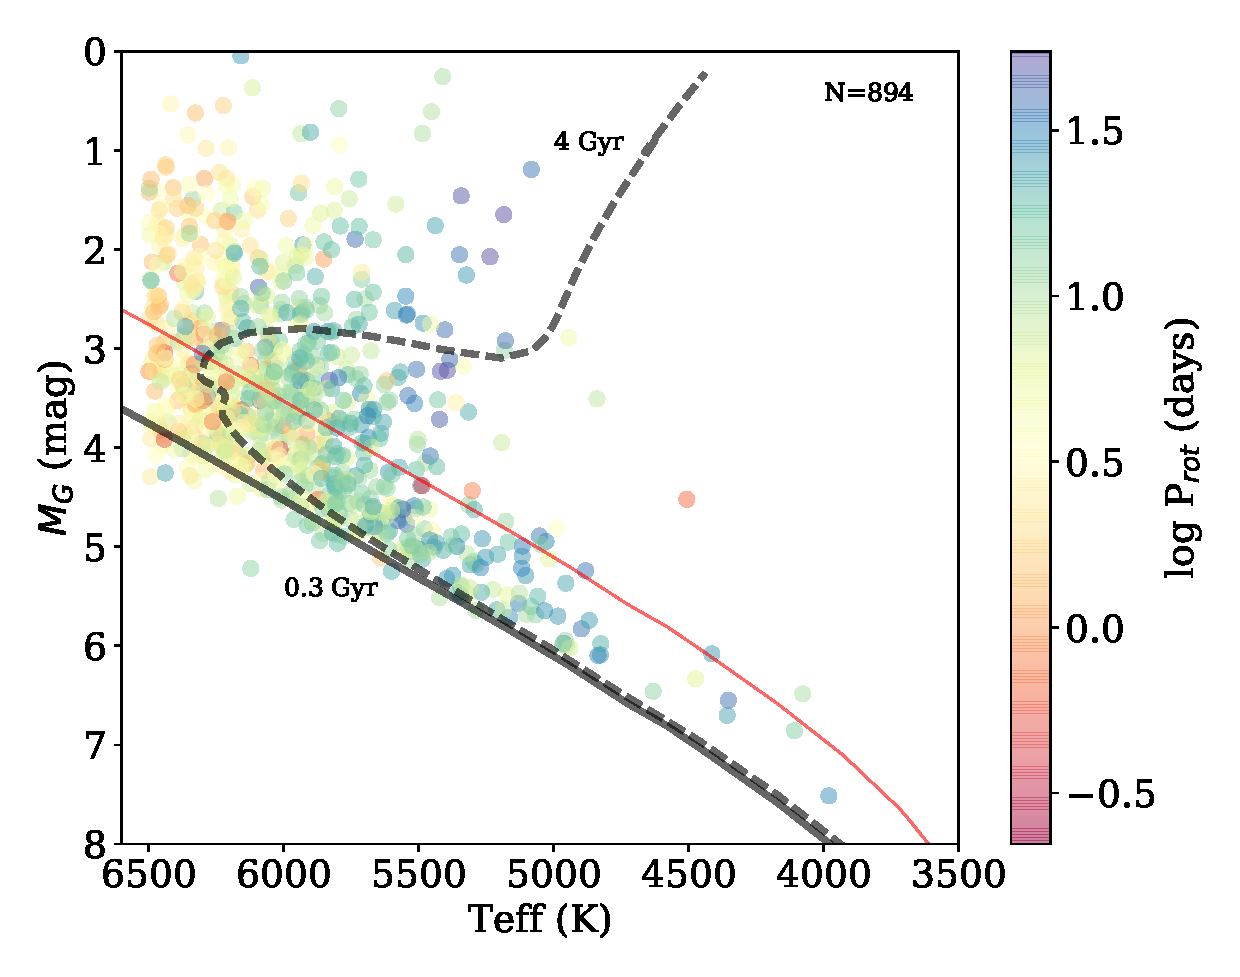
\includegraphics[width=3.5in]{davenport2016_fig2}
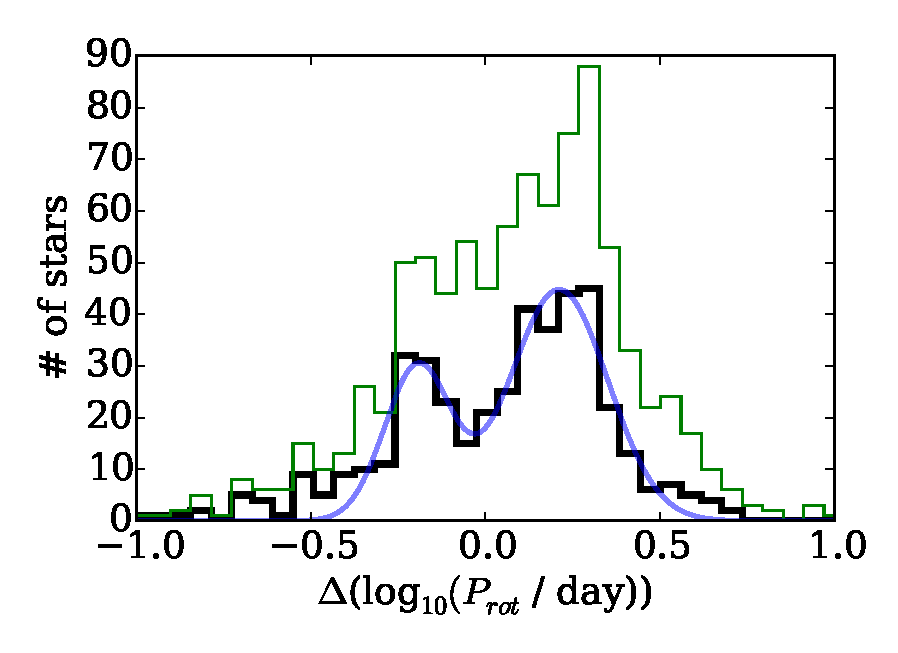
\includegraphics[width=3in]{davenport2016_fig4}
}
\caption{Left -- Figure 2 from \citet{davenport2017}, showing the absolute Gaia magnitude versus temperature for \Kepler stars with known rotation periods in the Gaia DR1 catalog. Sub-giant stars can be separated from main sequence targets using isochrone models (black solid \& dashed lines). Right -- Figure 4 from \citet{davenport2017}, showing the rotation period distribution relative to a 600 Myr ``gyrochrone'' before (green line) and after (black line) filtering our sub-giants. The bimodal distribution is apparent, and fit with a 2-Gaussian model (blue line).}
\label{fig:cmd}
\end{figure}




%%%%%%%%%
\subsection{Mapping Ages in each Field}
our catalog of rotation periods from K2, combined with existing catalogs from Kepler, we will have the largest set of rotation periods ever to use for population analysis. using new technique being developed by Ruth (Chronometer) we will have improved age estimate for every star based on single rotation values. then we combine this to get age distribution within each K2 field.

Demonstration figure?

discussion of improved gyrochronology calibration?

this is partially an extension of the period bimodality work (if it's an age effect), but to create a detailed map of the ages of these field stars at a range of galactic latitudes in the 17 pencil-beams available from K2. combining with the periods from Kepler, will be even better. ultimately we'd like to compare to the age distributions in simulations of these fields from TRILEGAL, and from other age indicators (asteroseismology, flare ages, etc)



%%%%%%%%%%%%%%%%%%%
\section{Team Qualifications}
PI Davenport has used \Kepler to conduct the largest survey to-date of stellar activity from flares, as well as multiple investigations of starspots and their evolution with time using \Kepler data. From these studies, Davenport has developed an age model for flare activity that will be directly comparable to the ages and starspot amplitudes derived from this study. He has also recently discovered the rotation period bimodality first noted with \Kepler M dwarfs by \citet{mcquillan2013} extends to G and K dwarf stars \citep{davenport2017}.
Davenport previously collaborated on NASA ADP grant NNX09AC77G to characterize NIR variability using the 2MASS Calibration Scan Point Source Working Database \citep{davenport2012,davenport2015a}.
He has mentored numerous students on projects using \Kepler data, resulting in student-led publications such as the flare activity of a unique M dwarf binary system GJ 1245AB \citep{lurie2015}, and exploring the poorly understood origins of wide binary stars through stellar rotation (R. Clarke in prep). He will manage the overall project, and lead the investigation and publication of the period bimodality exploration.

Co-I Angus is an expert in the extraction of periodic signals from \Kepler data using Gaussian Processes \citep{angus2016c} and other cutting-edge statistical techniques. She is the author of tools for generating Systematics-Insensitive Periodograms for both \Kepler and K2 data \citep{angus2016}, as well as new gyrochronology calibrations using \Kepler asteroseismic targets \citep{angus2015}. She will lead the effort to measure and publish rotation periods for all K2 sources, and lead the graduate student in measuring ages for field stars.

Covey

Kipping

Agueros

%%%%%%%%%%%%%%%%%%%
\section{Relevance to NASA Programs}
history of MWY, age of planet systems, TESS



%%%%%%%%%%%%%%%%%%%
\section{Plan of Work}
{\bf Year 1:} process all rotation period data
\\
{\bf Year 2:} write papers



\clearpage
%\pagestyle{empty}

\bibliography{/Users/james/Dropbox/references}


\end{document}

